\chapter{Modelo de señal y generación de eventos Monte Carlo}
\label{cap:simulaciones}

En este capítulo se describe como fueron simulados los procesos del modelo de
SUSY (\cref{sec:sig_samples}) y los procesos del SM (\cref{sec:bkg_samples}) que
dan lugar al estado final de interés. Todas las muestras fueron simuladas
utilizando generadores Monte Carlo a $\sqrt{s}=8\tev$, y a continuación se simuló
el pasaje por el detector ATLAS para luego ser reconstruidas con los mismos
algoritmos que los datos observados.

%% Todas las muestras fueron pasadas a través de la simulación completa basada en Geant4\cite{Geant4,AtlasSim} o rápida
%% ATLFAST-II\cite{Richter-Was:683751} del detector ATLAS, y reconstruidas con los mismos algoritmos
%% que se utilizaron para los datos.


\hll{Explicar mejor que significa un evento}
\hll{Estan los slha publicos? Citar HEPDATA}



\section{Simulación de la señal de SUSY}\label{sec:sig_samples}

Como se ha mencionado en el \cref{cap:susy}, debido al gran número de parámetros
libres en los modelos de SUSY, las búsquedas de supersimetría en ATLAS están
impulsadas por la fenomenología de los estados finales. El análisis realizado
para esta Tesis está motivado por estados finales con fotones energéticos,
provenientes del decaimiento de un neutralino NLSP en el contexto de modelos
GGM.

En los modelos GGM el decaimiento de los estados supersimétricos producidos en
las colisiones del LHC van a proceder por medio de decaimientos en cascada hasta
el neutralino NLSP que decaerá a un gravitino y una partícula del SM, que
dependerá de la naturaleza de la NSLP. Distintas posibilidades para la
naturaleza de la NLSP pueden ser consideradas, las cuales dan lugar a estados
finales distintos y complementarios entre si, para cubrir las distintas regiones
del espacio de fase de los modelos GGM. Dentro de ATLAS se exploraron cuatro
estados finales diferentes: dos fotones, un fotón y un leptón, un fotón y
{\bjets}, y un fotón y jets, todos con energía faltante, correspondiente a los
gravitinos LSP.

En particular en esta Tesis se focalizó en el análisis de un estado final que
consiste en un único fotón, jets y energía faltante.
La selección de eventos que se describe en el \cref{cap:seleccion} fue diseñada para
maximizar la sensibilidad a pequeñas señales con esta topología general.
Cualquier imposición de cortes muy dependientes del modelo fueron evitadas,
tratando de mantener el análisis lo mas independiente del modelo como fuera
posible. Sin embargo, una interpretación en el marco de un modelo especifico es
inevitable. Con tal motivo se simuló un conjunto de puntos de señal con
distintos valores de los parámetros para cubrir la región del espacio de
parámetros donde pueda manifestarse dicha señal.

%% Se simularon puntos de senal para la produccion de gluinosLos resultados se interpretaron
%% son interpretados en el contexto de GGM que
%% incluyen la produccion de supercompaneras de particulas del SM que se acoplan
%% fuertemente comot ambien de que poseen solo carga electrodebil.

Se utilizó un espectro simplificado en el cual, básicamente, el espacio de
parámetros consiste en la escala de producción (por simplicidad, la masa del
gluino) y la masa de la NLSP. Todos los demás estados fueron desacoplados ya que
no juegan un rol importante en la producción o en el estado final de interés.
Esta aproximación es similar a los denominados \emph{modelos simplificados}
utilizados en otras búsquedas.
La masa del gluino es el único parámetro libre de las partículas de color para
poder determinar un límite conservativo en la masa del mismo. Todos los
parámetros de masa soft de los squarks se fijan en 2.5 \tev.

Para maximizar la probabilidad de tener un único fotón en el estado final, es
necesario que $\mathrm{BR}(\ninoone \to \gam\,\gravino) \sim 50\%$. Esto resulta
cuando el neutralino más liviano es una mezcla bino-higgsino.
Además, el valor de $\mu$ debe ser positivo para
suprimir el decaimiento a Higgs, que llevará a un estado final ya cubierto por
otro análisis de ATLAS.
Para lograr la BR
deseada se variaron los parámetros de
masa de bino ($M_1$) y higgsinos ($\mu$) para las diferentes masas del {\ninoone}, de tal forma que los BR del {\ninoone}
sean aproximadamente constantes:

\begin{align}
  &\mathrm{BR}(\ninoone \to \gam\, \gravino) \approx 50\% \label{eq:n1_gam}\\
  &\mathrm{BR}(\ninoone \to Z\, \gravino) \approx 49\%    \label{eq:n1_z} \\
  &\mathrm{BR}(\ninoone \to h\, \gravino) \approx 1\%     \label{eq:n1_h}
\end{align}


Los demás parámetros del modelo se fijan en $M_2=2.5\tev$, $\tan\beta=1.5$ y
$c\tau_{\mathrm{NLSP}} < 0.1$ mm. Este último asegura que el neutralino decaiga
rápidamente dentro del detector y se logra haciendo al gravitino lo
suficientemente liviano ($m_{\tilde{G}}=10^{-9} \gev$). Todos los términos
tri-lineares son fijados a cero y las masas de los sleptones a $2.5 \tev$.
Las masas del higgs liviano ($h$) y el pseudoescalar ($A$) se fijan a
$m_{h} = 126 \gev$ y $m_{A} = 2 \tev$.
La masa del $h$ se considera a partir del valor
medido de la masa del Higgs observado en el a\~no 2012.
En modelos GGM de SUSY existen distintos
mecanismos\cite{Craig:2011yk,Auzzi:2011eu,Csaki:2012fh,Larsen:2012rq,Craig:2012hc}
para generar una masa del bosón de Higgs tan alta como este valor observado, sin
cambiar la fenomenología de los modelos considerados. No se observó un efecto
significativo en el espectro de masas variando el valor de la masa de Higgs en un
rango de $\pm 10 \gev$.
%% Tambien se estudio el efecto de variar el valor
%% de $\tan\beta$\note{Hacer comentario de $\tan\beta$}

A partir de estos estudios se procedió a simular un conjunto de puntos de señal
(grid) en el plano ($m_{\gluino}$, $m_{\ninoone}$), variando los parámetros
$M_3$ y $\mu$. El parámetro $M_1$ se ajustó, dependiendo del $\mu$ de forma de
obtener las BR descriptas anteriormente. La grid cubre el espacio $150\gev <
m_{\ninoone} < 1250 \gev$ y $800\gev < m_{\gluino} < 1300 \gev$, con
$m_{\ninoone} < m_{\gluino}$ (ver \cref{fig:gridpoints}).


\begin{figure}[!htb]
  \centering
  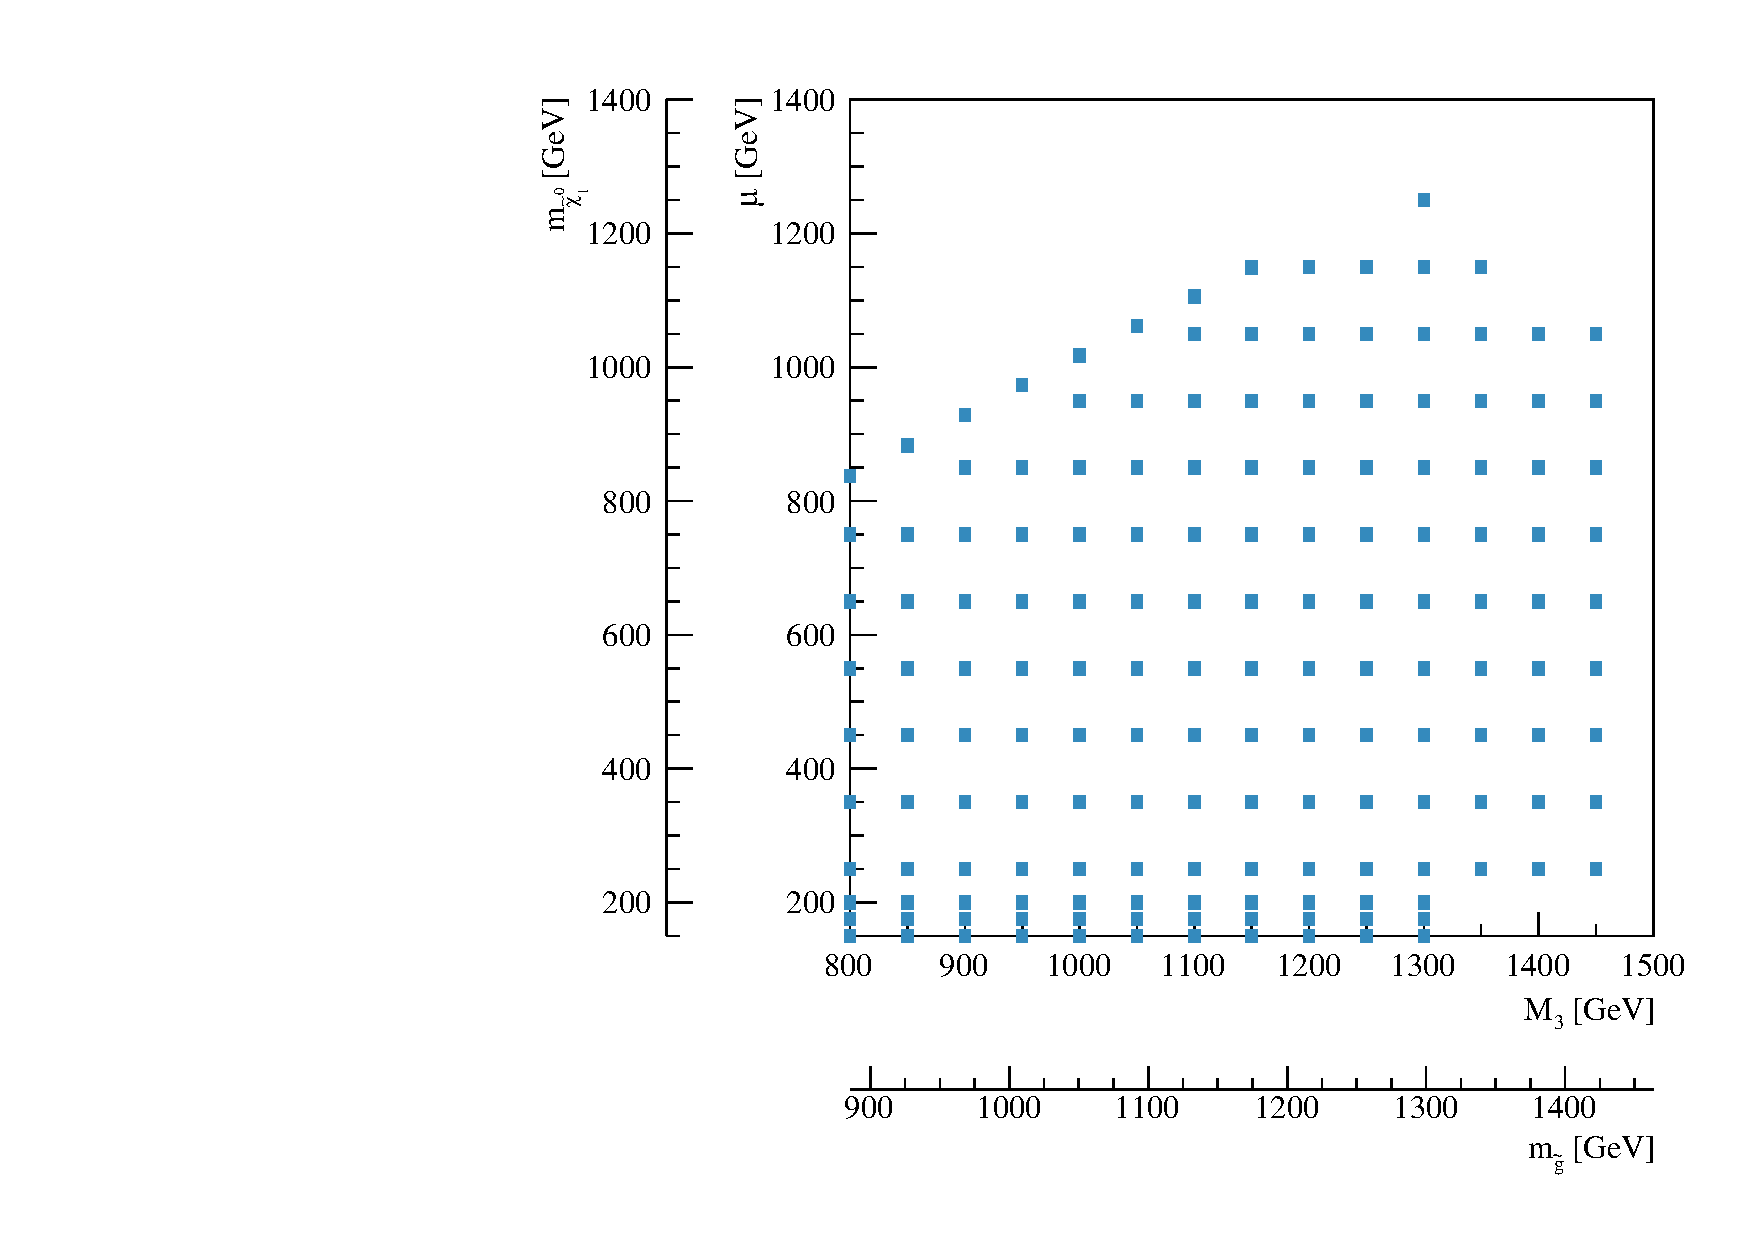
\includegraphics[width=0.9\textwidth]{figures/run1_grid}
  \caption{Conjunto de puntos (grid) de señal simulada para el presente análisis. Los cuadrados azules representan los distintos puntos
  de señal generados con distintos valores de $m_{\gluino}$ y $m_{\ninoone}$. También puede verse la relación con las masas $m_{\gluino}$ y $m_{\ninoone}$.}
  \label{fig:gridpoints}
\end{figure}


El espectro completo de masas y los correspondientes decaimientos fueron
calculados a partir de estos parámetros utilizando {\suspect}
(v2.41)\cite{Djouadi2007426}, {\sdecay} (v1.3b)\cite{Muhlleitner:2004mka} y
{\hdecay} (v3.4)\cite{Djouadi:1997yw}, que forman parte del paquete {\susyhit}
(v1.3)\cite{Djouadi:2006bz}. Algunos ejemplos del espectro de masas pueden verse
en la \cref{fig:mass_spectra}, para algunos puntos de la grid, (xx y yy).

\begin{figure}[!htb]
   \centering
   \includegraphics[width=0.45\textwidth]{figures/masses_GGM_M3_mu_800_150}
   %%\includegraphics[width=0.45\textwidth]{figures/masses_GGM_M3_mu_1000_750}
   \includegraphics[width=0.45\textwidth]{figures/masses_GGM_M3_mu_1450_1050}

   \caption{Espectro de masas de las particulas supersimetricas para dos puntos de la grid de senal.
     En la izquierda para XXX y en la derecha XXX.}
     %% Solo $M_3$ y $\mu$ son los parámetros libres, en este caso
     %% $(M_3, \mu) = (800~\gev, 250~\gev)$. }
   \label{fig:mass_spectra}
\end{figure}

Para cada uno de los 124 puntos de señal que constituyen la grid se generaron
5000 eventos, utilizando {\herwigpp} v2.5.2\cite{Bahr:2008pv} y el conjunto de
PDFs CTEQ6L1\cite{Nadolsky:2008zw}. Se aplicó un filtro a nivel generador, que
requería la presencia de un fotón con un {\pt} de al menos 100 \gev, para
optimizar la generación, especialmente en los puntos donde el
neutralino tiene menor masa. La eficiencia del filtro para todas las muestras
simuladas puede verse en la \cref{tab:signal_filter_eff}. La simulación del
detector ATLAS se realizó con la simulación rápida
\textsc{ATLFAST-II}\cite{Richter-Was:683751}.


\begin{table}[!htb]
  \centering
  \caption{Relación entre los parámetros libres del modelo $M_3$ y $\mu$ con las
    masas $m_{\gluino}$ (izquierda) y $m_{\ninoone}$ (derecha), respectivamente.
    En la tabla de la derecha, para cada valor de $\mu$ también se puede
    observar el valor de $M_1$ utilizado para obtener los BR de decaimiento del
    {\ninoone} deseados.}
  \label{tab:signal_pars}

  \begin{minipage}[!t]{0.5\textwidth}
    \centering
    \begin{tabular}{cc}
      \hline
      $M_3$ [\gev]& $m_{\gluino}$ [\gev] \\
      \hline
      800  & 885.5 \\
      850  & 931.7 \\
      900  & 977.6 \\
      950  & 1023.1 \\
      1000 & 1068.3  \\
      1050 & 1113.3  \\
      1100 & 1157.9  \\
      1150 & 1202.3  \\
      1200 & 1246.4  \\
      1250 & 1290.3  \\
      1300 & 1333.9  \\
      1350 & 1377.3  \\
      1400 & 1420.5  \\
      1450 & 1463.4  \\
      \hline
    \end{tabular}
    \vspace{5cm}
  \end{minipage}%
  \begin{minipage}[t]{0.5\textwidth}
    \begin{tabular}{ccc}
      \hline
      $\mu$ [\gev] & $M_1$ [\gev] & $m_{\ninoone}$ [\gev] \\
      \hline
      150  &  300  & 147.0 \\
      175  &  270  & 168.3 \\
      200  &  267  & 190.3 \\
      250  &  288  & 235.8 \\
      350  &  365  & 332.4 \\
      450  &  456  & 433.2 \\
      550  &  551  & 535.6 \\
      650  &  647  & 638.3 \\
      750  &  745  & 742.0 \\
      838  &  837  & 836.4 \\
      850  &  845  & 846.7 \\
      883  &  882  & 883.7 \\
      928  &  926  & 930.2 \\
      950  &  942  & 949.6 \\
      973  &  970  & 976.6  \\
      1017 &  1015 & 1023.4 \\
      1050 &  1040 & 1053.0 \\
      1062 &  1058 & 1068.9 \\
      1106 &  1102 & 1114.8 \\
      1149 &  1145 & 1160.0 \\
      1150 &  1140 & 1157.5 \\
      1250 &  1238 & 1260.6 \\
      \hline
    \end{tabular}

  \end{minipage}

\end{table}



%% \M{1} and $\mu$ determine the lightest neutralino mass, and are related in such a way that the branching ratios of the \ninoone\ are approximately constant,
%% resulting in ${\rm BR}(\ninoone \to \gam + \gravino) \approx 50\%$, ${\rm BR}(\ninoone \to Z + \gravino) \approx 49\%$ and ${\rm BR}(\ninoone \to h + \gravino) \approx 1\%$,
%% numbers which vary by $\pm 1\%$ throughout most of the grid ({\fig} \ref{fig:br_n1_x_grav}). For light neutralinos ($<200\gev$) the Higgs production is highly
%% suppressed and ${\rm BR}(\ninoone \to \gam + \gravino)$ starts falling up to 40\%. The value of $\mu$ must also be positive in order to disfavor the branching ratio
%% to the Higgs boson, which would lead to a signature already covered by a dedicated analysis in ATLAS \cite{Aad:2012jva}. Similarly, the branching ratio for
%% ($\ninoone \to \gam + \gravino$) is such that maximizes the single photon final state. At larger values the diphoton topology starts to be favoured, which has been
%% extensively searched for in the past \cite{Aad2012519,Aad:2011kz}. This leaves $M_3$ and $\mu$ as the only two free parameters of the model, spanning the space
%% within $150\gev < m_{\ninoone} < 1250 \gev$ and $800\gev < m_{\gluino} < 1300 \gev$, with $m_{\ninoone} < m_{\gluino}$. The granularity of the simulation in each
%% dimension is shown in {\tab}\ \ref{tab:signal_pars}, with the resulting value for the gluino and neutralino masses.




%%The total decay branching ratios for \gluino-initiated \ninoone\ production are
%% shown in {\fig} \ref{fig:br_gl_n1}, for 2-body\footnote{only effectively, the gluino decays through a virtual
%% quark-squark loop in this case.} and 3-body gluino decays.


\begin{table}[ht]
  \centering
  %\small
  \footnotesize
  \caption{Eficiencia del filtro a nivel generador [\%]
    para los puntos de señal simulados.}
  \begin{tabular}{c|ccccccccccccccccc}
    \hline
%       &    \multicolumn{11}{c}{Filter efficiency [\%]} \\
%	\hline
     &   \multicolumn{14}{c}{ $M_3$ [\gev] } \\
    $\mu$ [\gev] &  800 & 850 & 900 & 950 & 1000 & 1050 & 1100 &1150 & 1200  & 1250 & 1300 & 1350 & 1400 & 1450 \\
    \hline
    150  &   39.54 &   39.8 &  41.9    &   42.6   &   43.0   &   44.2   &   45.5    &   46.3    &    47.1  &   48.3  &   49.1 &      &      &       \\
    175  &   44.55 &   44.6 &  46.5    &   47.5   &   47.8   &   48.9   &   50.3    &   51.4    &    51.5  &   52.4  &   53.3 &      &      &       \\
    200  &   47.66 &   48.4 &  50.1    &   50.6   &   52.0   &   52.8   &   53.8    &   55.0    &    55.0  &   56.2  &   56.0 &      &      &       \\
    250  &   55.09 &   56.0 &  56.1    &   57.1   &   56.7   &   58.0   &   58.9    &   59.5    &    60.5  &   60.7  &   61.2 & 62.1 & 62.2 &  63.9 \\
    350  &   65.82 &   66.1 &  64.6    &   65.8   &   66.4   &   66.7   &   66.5    &   67.7    &    67.4  &   67.6  &   67.8 & 68.0 & 69.2 &  68.4 \\
    450  &   71.29 &   71.4 &  71.4    &   71.8   &   72.1   &   72.5   &   72.0    &   72.6    &    72.1  &   72.5  &   73.4 & 72.9 & 72.2 &  73.4 \\
    550  &   73.08 &   72.5 &  73.3    &   73.7   &   74.6   &   74.3   &   75.0    &   74.8    &    74.2  &   74.7  &   75.6 & 75.7 & 74.9 &  75.3 \\
    650  &   69.78 &   72.0 &  73.2    &   74.1   &   75.6   &   76.2   &   75.9    &   75.8    &    77.0  &   77.0  &   76.2 & 76.7 & 77.1 &  76.6 \\
    750  &   47.69 &   60.2 &  66.9    &   70.4   &   73.4   &   74.0   &   75.9    &   76.5    &    77.1  &   77.3  &   76.3 & 77.9 & 77.2 &  77.0 \\
    838  &    9.0  &        &          &          &          &          &           &           &          &         &        &      &      &       \\
    883  &         &   9.1  &          &          &          &          &           &           &          &         &        &      &      &       \\
    850  &         &        &  34.2    &   50.7   &   60.1   &   66.4   &   70.4    &   73.5    &    73.6  &   75.4  &   76.6 & 77.1 & 78.2 &  76.8 \\
    928  &         &        &   9.4    &          &          &          &           &           &          &         &        &      &      &       \\
    950  &         &        &          &          &   25.4   &   41.4   &   54.0    &   62.2    &    66.8  &   70.9  &   75.2 & 75.9 & 78.1 &  77.2 \\
    973  &         &        &          &   10.0   &          &          &           &           &          &         &        &      &      &       \\
    1017 &         &        &          &          &   10.3   &          &           &           &          &         &        &      &      &       \\
    1050 &         &        &          &          &          &          &   19.2    &   31.6    &    45.2  &   56.8  &   62.7 & 68.9 & 73.1 &  75.6 \\
    1062 &         &        &          &          &          &   11.1   &           &           &          &         &        &      &      &       \\
    1106 &         &        &          &          &          &          &   11.7    &           &          &         &        &      &      &       \\
    1149 &         &        &          &          &          &          &           &   12.6    &          &         &        &      &      &       \\
    1150 &         &        &          &          &          &          &           &           &    16.1  &   24.9  &   36.9 & 49.0 &      &       \\
    1250 &         &        &          &          &          &          &           &           &          &         &   16.1 &      &      &       \\
    \hline
  \end{tabular}
  \label{tab:signal_filter_eff}
\end{table}



\subsection{Estudios a nivel generador.} %% \hl{Cambiar nombre...}}
\label{sec:susy_studies}

Se realizaron algunos estudios para entender mejor el estado final y poder
identificar las distintas regiones en el espacio de fase, lo cual facilitaría el
proceso de optimización de las posibles regiones de se\~nal. En la
\cref{fig:signal_br_gl} se presentan los distintos BR de los gluinos para todos
los puntos de la grid. Resulta evidente que la cadena de decaimiento dominante
varía en las distintas regiones de la grid, dependiendo de la masa del gluino y
el neutralino. Se puede ver que el decaimiento dominante es a través de
charginos, pero a medida que la masa del gluino y el neutralino se acercan,
empieza a resultar más importante el decaimiento directo al neutralino más
liviano, mientras que en los puntos más cercanos a la diagonal, el decaimiento
estará dominado por $\gluino\to g\gravino$ el cual no corresponde al estado
final deseado. Los diagramas de los distintos decaimientos posibles se encuentran
en la \cref{fig:signal_diagrams}, de los cuales se pueden extraer varias
conclusiones: en el caso de las cadenas largas a través de charginos, el estado
final tendrá una mayor cantidad de jets. Si el decaimiento es directamente al
{\ninoone} la multiplicidad de jets será menor y la energía del fotón será mayor
al igual que la energía faltante.


\begin{figure}[!htb]
  \centering

  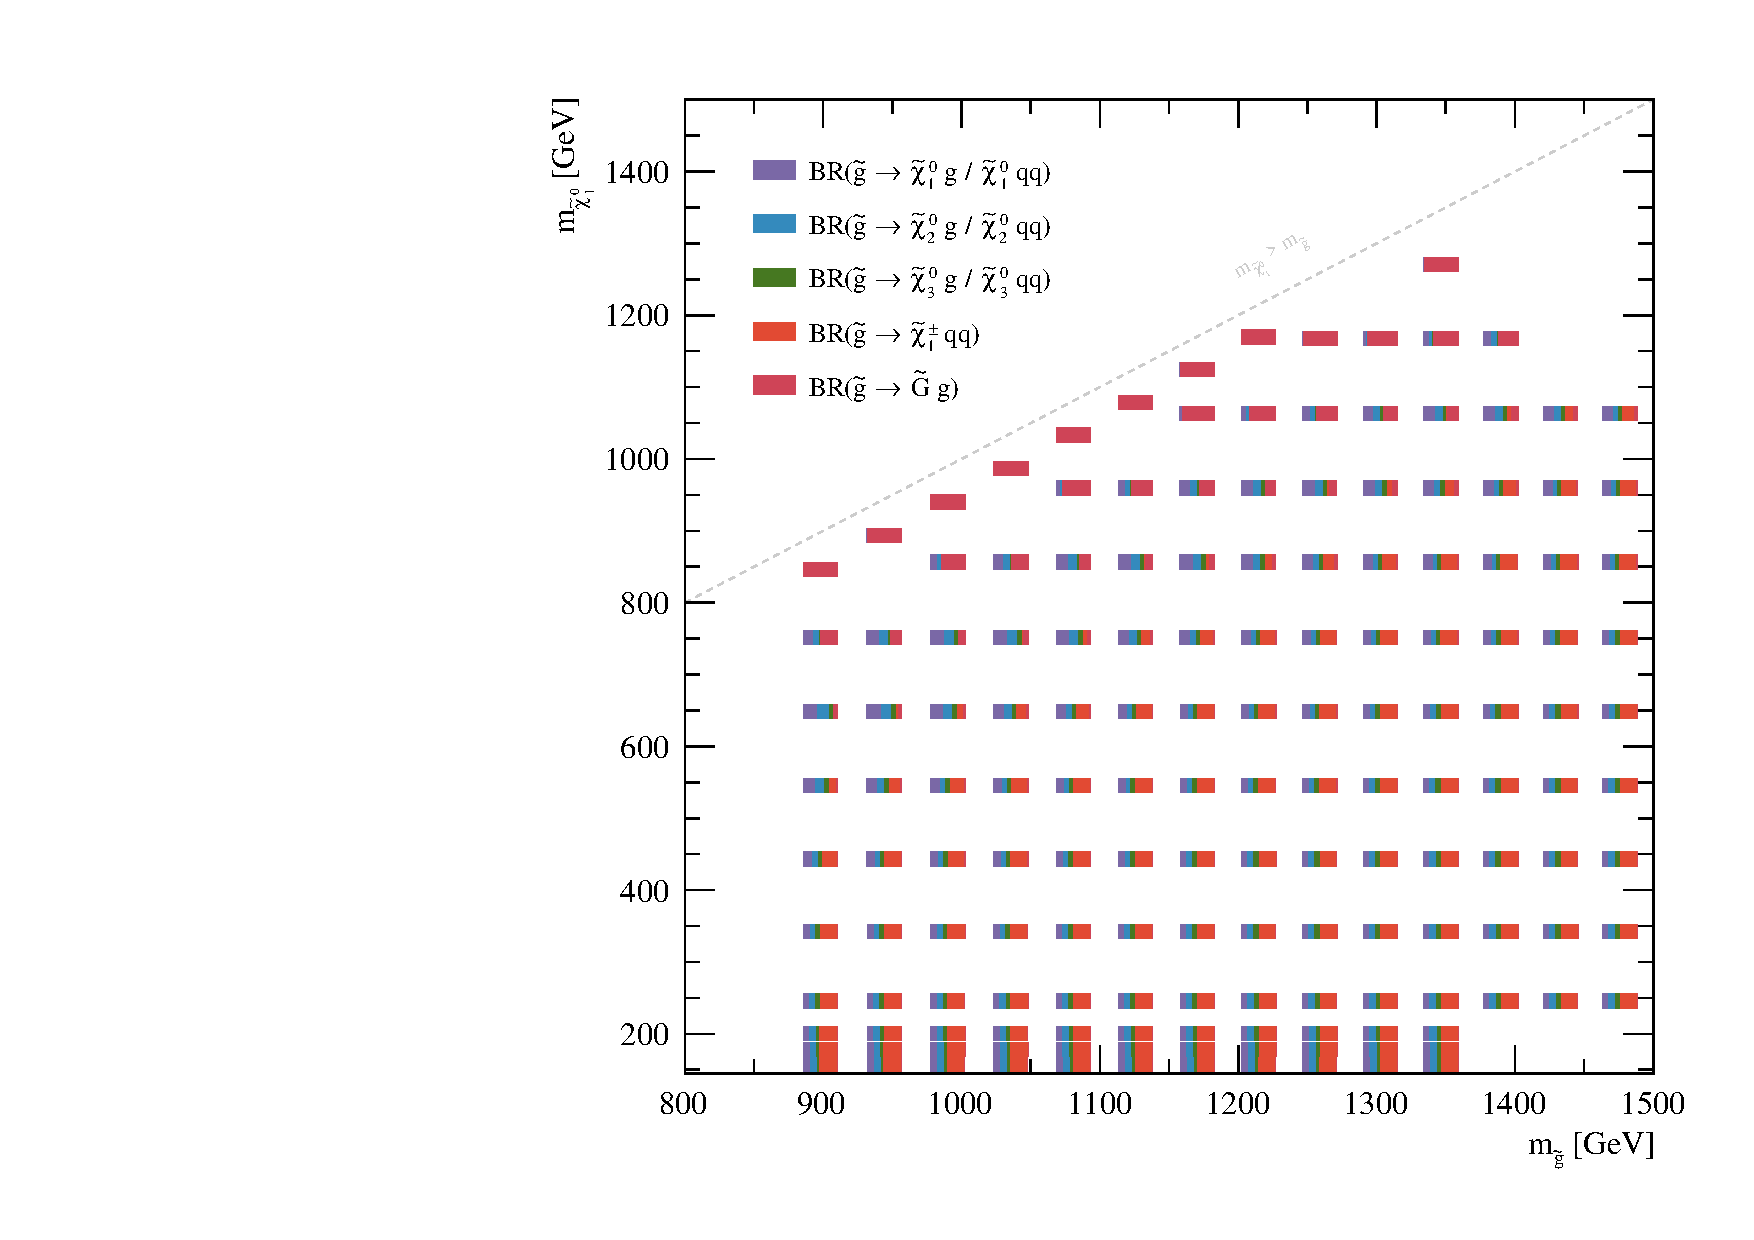
\includegraphics[width=0.9\textwidth]{figures/br_gl_X}

  \caption{Tasas de decaimiento (BR) de los gluinos para los distintos puntos de la grid en
    el plano \mgmn.}
  \label{fig:signal_br_gl}
\end{figure}


\begin{figure}[!htb]
  \centering

  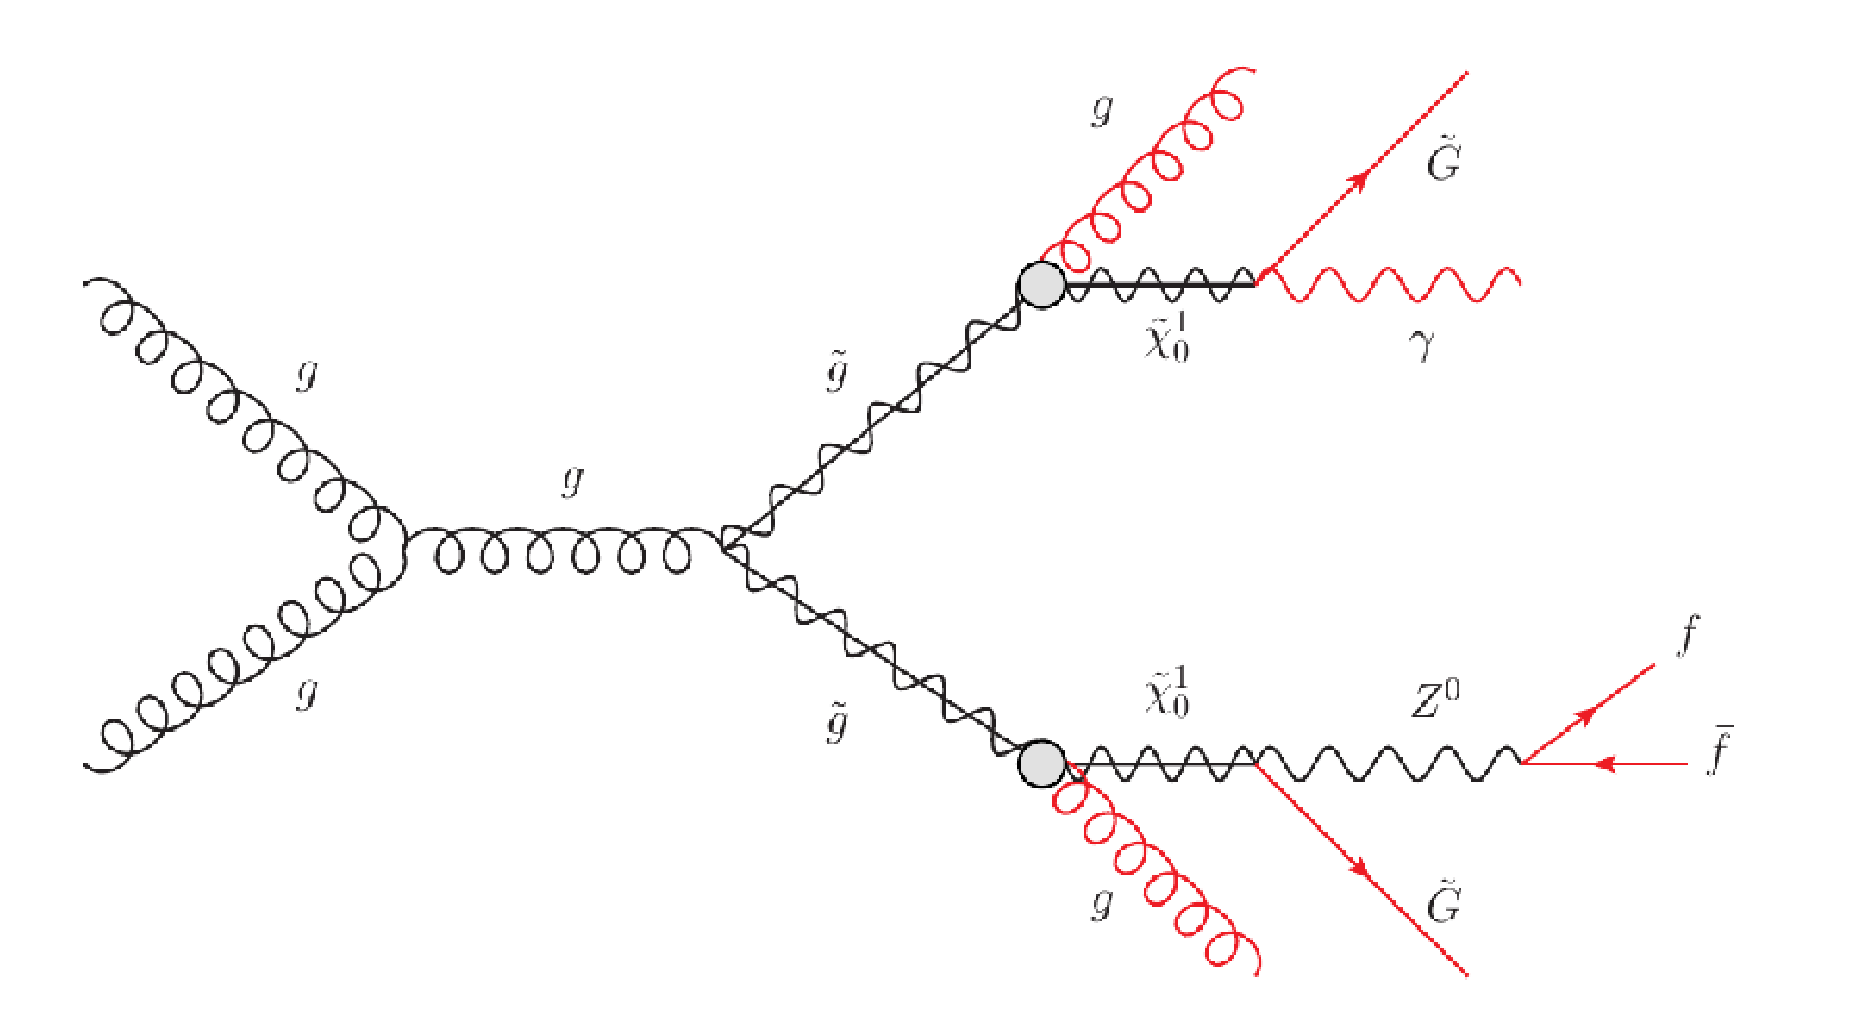
\includegraphics[width=0.49\textwidth]{diagram_a}
  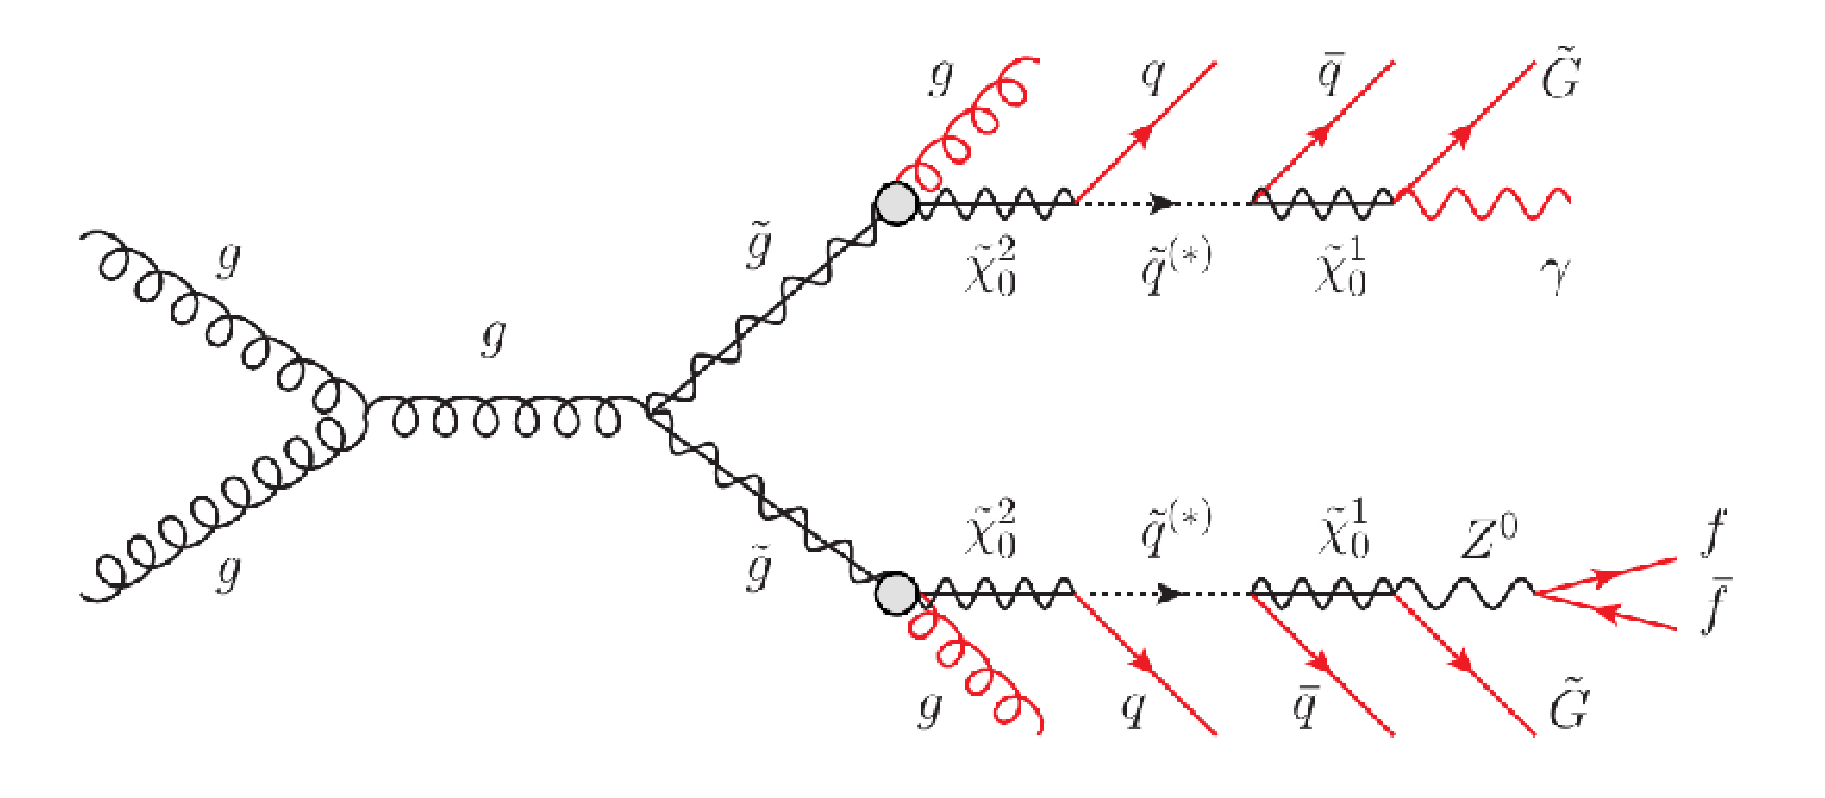
\includegraphics[width=0.49\textwidth]{diagram_b}

  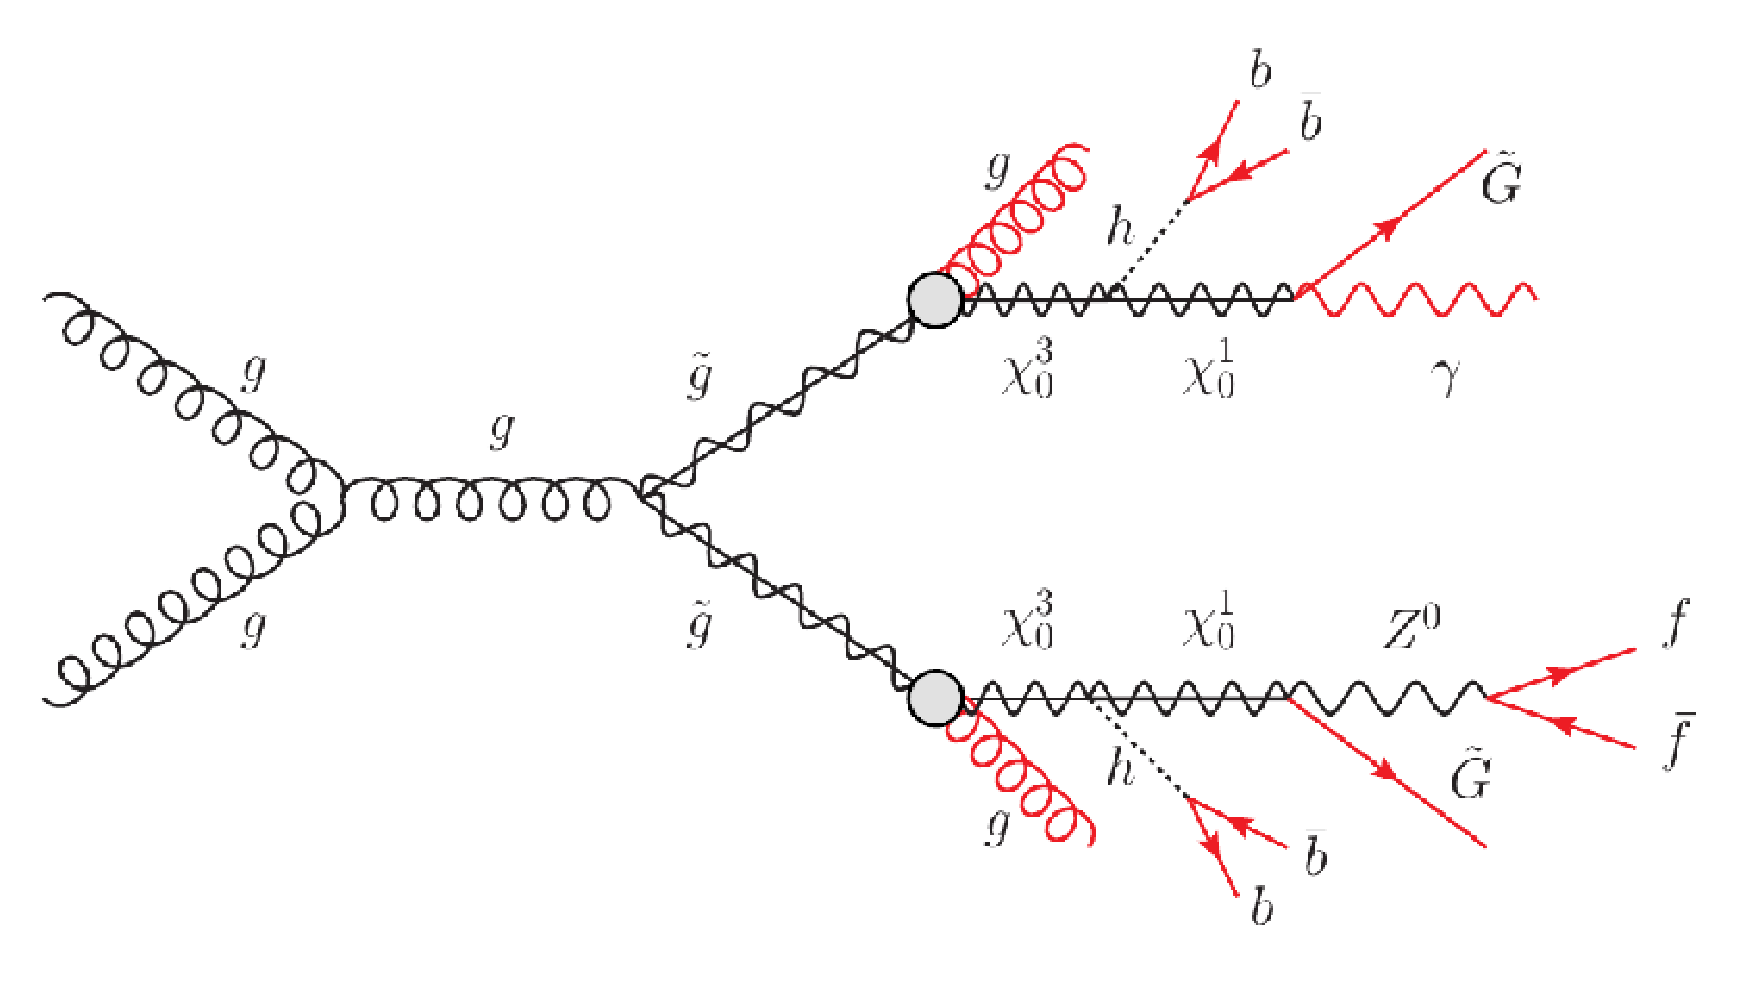
\includegraphics[width=0.49\textwidth]{diagram_c}
  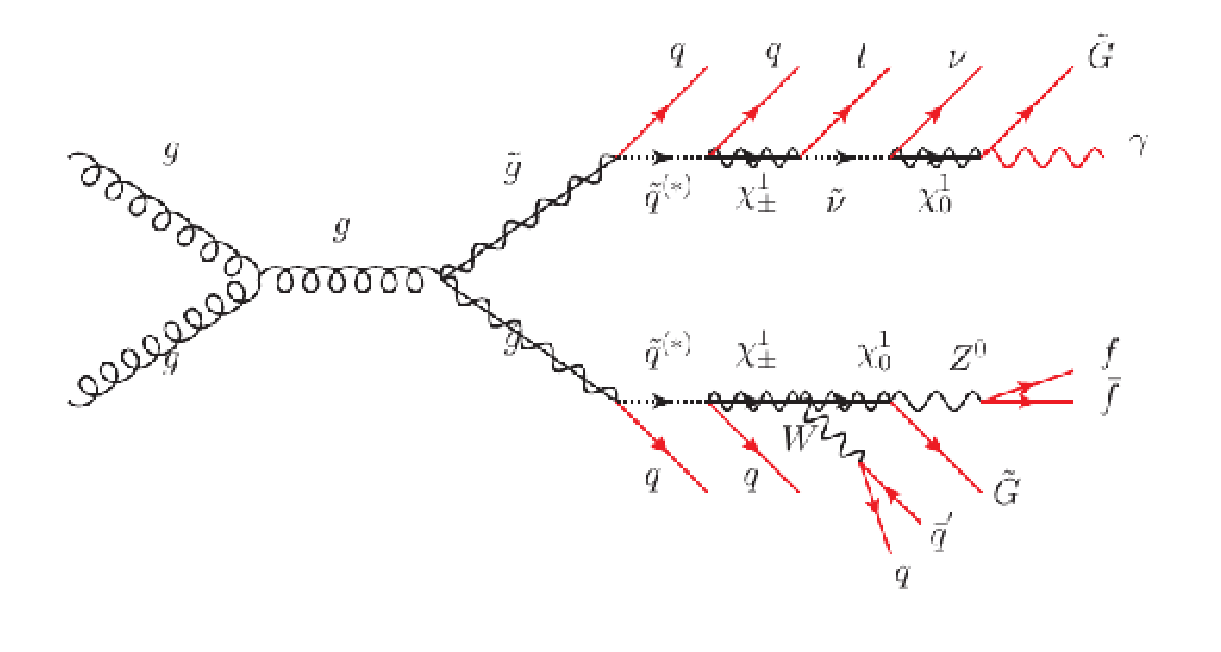
\includegraphics[width=0.49\textwidth]{diagram_d}

  \caption{Diagramas de Feynman para la producción de gluinos y el subsiguiente
    decaimiento de los mismos hasta el estado final. Los distintos diagramas ilustran \hl{...} }
  \label{fig:signal_diagrams}

\end{figure}


En la \cref{fig:signal_br_n1} se presentan las BR de decaimiento del neutralino
mas liviano (\ninoone), compatibles con las esperadas a partir del modelo que se
utilizará para el presente analisis (\cref{eq:n1_gam,eq:n1_z,eq:n1_h}). Estos
valores varían en menos del 1\% en los distintos puntos de la grid, salvo para
neutralinos livianos ($<200\gev$) donde la producción de Higgs es altamente
suprimida, mientras aumenta el decaimiento a $Z$, y $\mathrm{BR}(\ninoone \to
\gam \gravino)$ empieza a caer llegando al 40\%.

\begin{figure}[!htb]
  \centering

  \includegraphics[width=0.9\textwidth]{figures/br_n1_X}

  \caption{Tasas de decaimiento (BR) de los neutralinos LSP en $\gamma\gravino$, $\gamma Z$ y
  $\gamma h$ para los distintos puntos de la grid en el plano \mgmn.}
  \label{fig:signal_br_n1}
\end{figure}





%% \begin{figure}[h]
%%   \centering
%%   \includegraphics[width=0.8\textwidth]{figures/truth/br_gl_2b_vs_3b}
%%   \caption{BR de los gluinos para los distintos puntos de la grid.}
%% \end{figure}

%% \begin{figure}[h]
%%   \includegraphics[width=0.8\textwidth]{figures/truth/br_gl_X_2body}
%%   \includegraphics[width=0.8\textwidth]{figures/truth/br_gl_X_3body}
%%  \caption{BR de los gluinos para los distintos puntos de la grid.}
%% \end{figure}


%% \begin{figure}[h]
%%   \centering
%%   \includegraphics[width=0.8\textwidth]{figures/truth/br_c1_X}
%%   \caption{BR de los gluinos para los distintos puntos de la grid.}
%% \end{figure}

%% \begin{figure}[h]
%%   \centering
%%   \includegraphics[width=0.8\textwidth]{figures/truth/br_n3_X}
%%   \caption{BR de los gluinos para los distintos puntos de la grid.}
%% \end{figure}

%% \begin{figure}[h]
%%   \centering
%%   \includegraphics[width=0.8\textwidth]{figures/truth/br_n2_X}
%%   \caption{BR de los gluinos para los distintos puntos de la grid.}
%% \end{figure}

%% \begin{figure}[h]
%%   \centering
%%   \includegraphics[width=0.8\textwidth]{figures/truth/br_n1_X}
%%   \caption{BR de los gluinos para los distintos puntos de la grid.}
%% \end{figure}


%% \begin{figure}[ht!]
%%    \centering
%%    \includegraphics[width=0.32\textwidth]{figures/gl_n1g_full}
%%    \includegraphics[width=0.32\textwidth]{figures/gl_n1qq_full}
%%    \includegraphics[width=0.32\textwidth]{figures/gl_n1_full} \\
%%    \includegraphics[width=0.32\textwidth]{figures/gl_n2g_full}
%%    \includegraphics[width=0.32\textwidth]{figures/gl_n2qq_full}
%%    \includegraphics[width=0.32\textwidth]{figures/gl_n2_full} \\
%%    \includegraphics[width=0.32\textwidth]{figures/gl_n3g_full}
%%    \includegraphics[width=0.32\textwidth]{figures/gl_n3qq_full}
%%    \includegraphics[width=0.32\textwidth]{figures/gl_n3_full} \\
%%    \includegraphics[width=0.32\textwidth]{figures/gl_c1qq_full} \\

%%    \caption{Tasas de decaimiento para $\gluino \to \ninoone$,
%%      para todas las posibles cadenas de decaimiento permitidas en la grid
%%      de produccion fuerte. La mayoria de los graficos son la suma
%%      de deciamientos de 2 cuerpos (izquierda) y 3 cuerpos (centro).
%%      Para el decaimiento $\gluino \to \chinopm$), solo el decaimiento de
%%      tres cuerpos es posible.}
%%    \label{fig:br_gl_n1}
%% \end{figure}


\subsection{Sección eficaz de producción}
\label{sec:xs_calc}

%% La seccion eficaz de produccion y sus incertezas fue calculada usando el paquete SUSYSignalUncertainties \cite{SUSYsigunc}.
%% La seccione eficaz para los procesos que in volucran la produccion de pares de gluinos fueron calculadas a NLO
%% en la constante de acoplamiento fuerte, agregando la \hl{resummation of soft gluon emission at NLO+NLL}\cite{Beenakker:1996ch,Kulesza:2008jb,Kulesza:2009kq,Beenakker:2009ha,Beenakker:2011fu}.
%% La seccion eficas de produccion electrodebil de $\tilde{\chi}\tilde{\chi}$ fue calculada
%% a NLO en la constante de acoplamiento fuerte utilizando {\prospino} \cite{Beenakker:1999xh}.
%% Las secciones eficacez y sus incertezas estan detalladas en la \cref{tab:signal_xs_strong,tab:signal_xs_ewk}
%% y se muestran en las figuras...

En el caso de procesos de producción de pares de gluinos o squarks, de los cuales
existe el cálculo a NLL, la sección eficaz se toma a NLO en la constante de acoplamiento
fuerte, y se incluye la suma de la emisión de gluones soft con precisión NLL,
realizada utilizando {\nllfast}\cite{Kramer:2012bx,Beenakker:1996ch,Kulesza:2008jb,Kulesza:2009kq,Beenakker:2009ha,Beenakker:2011fu}.

En el caso de la producción de otro tipo de procesos, como la producción electrodébil de
partículas supersimétricas, se utilizan
las secciones eficaces calculadas a NLO usando {\prospino}.


\newcommand{\pdfcteqpm}{\ensuremath{\Delta\mathrm{PDF}^{\pm}(\mathrm{CTEQ})}}
\newcommand{\scacteqpm}{\ensuremath{\Delta\mathrm{SCA}^{\pm}(\mathrm{CTEQ})}}

\newcommand{\pdfmstwpm}{\ensuremath{\Delta\mathrm{PDF}^{\pm}(\mathrm{MSTW})}}
\newcommand{\scamstwpm}{\ensuremath{\Delta\mathrm{SCA}^{\pm}(\mathrm{MSTW})}}

\newcommand{\alphap}{\ensuremath{\alpha_s_+}}
\newcommand{\alpham}{\ensuremath{\alpha_s^-}}
\newcommand{\alphapm}{\ensuremath{\alpha_s^{\pm}}}

Las incertezas debidas a la elección de la escala de renormalización y
factorización como también aquellas asociadas a la PDF, son obtenidas utilizando {\nllfast} o
calculadas con {\prospino}. A fin de combinar todas estas predicciones y obtener
una incerteza total, se siguen las recomendaciones PDF4LHC\cite{Botje:2011sn}.
Para esto se define la envolvente de las predicciones a la sección eficaz usando
el intervalo a 68\% CL del conjunto de PDFs CTEQ (incluyendo la incerteza en
$\alpha_s$) y MSTW, junto con las variaciones de las escalas. La sección eficaz
nominal se obtiene usando el punto medio de la envolvente y la incerteza como la
mitad del ancho de la misma. Matemáticamente si {\pdfcteqpm} y {\scacteqpm} son
las variaciones en $\pm 1\sigma$ de las PDF CTEQ,  {\pdfmstwpm} y {\scamstwpm}
son las variaciones en $\pm 1\sigma$ en la PDF MSTW, y {\alphapm} son las
correspondientes incertezas de la constante de acoplamiento fuerte, entonces,

\begin{align}
  \Delta\mathrm{CTEQ}^{\pm} &= \sqrt{(\pdfcteqpm)^2 + (\scacteqpm)^2 + (\alphapm)^2} \\
  \Delta\mathrm{MSTW}^{\pm} &= \sqrt{(\pdfmstwpm)^2 + (\scamstwpm)^2}
\end{align}

Los correspondientes extremos por arriba y abajo de la envolvente pueden calcularse a partir de estos:

\begin{align}
  U &= \max(\Delta\mathrm{CTEQ}^\mathrm{nom} + \Delta\mathrm{CTEQ}^{+},\quad \Delta\mathrm{MSTW}^\mathrm{nom} + \Delta\mathrm{MSTW}^{+}) \\
  L &= \min(\Delta\mathrm{CTEQ}^\mathrm{nom} - \Delta\mathrm{CTEQ}^{-},\quad \Delta\mathrm{MSTW}^\mathrm{nom} - \Delta\mathrm{MSTW}^{-})
\end{align}
%
y la sección eficaz final ($\sigma$) y su incerteza simétrica ($\Delta\sigma$) se obtiene como:

\begin{equation}
  \sigma = (U+L)/2,\quad \Delta\sigma = (U-L)/2
\end{equation}


En la \cref{tab:signal_xs_strong} puede verse la sección eficaz de producción de
pares de gluinos para los distintos puntos de la grid de señal generada. La
sección eficaz de producción electrodébil de neutralinos/charginos se encuentra en la
\cref{tab:signal_xs_ewk}. En la \cref{fig:signal_xs} también se encuentra
graficada la sección eficaz como función de la masa de las partículas
producidas, mientras que en la \cref{fig:signal_xs_total} se puede apreciar la
fracción en la producción electrodébil comparada con la producción total.

\begin{table}[!htb]
  \centering
  \caption{Sección eficaz a NLO+NLL para la producción de gluinos para los distintos
    puntos de la grid de señal. La ultima columna es la incerteza teórica.}
  \begin{tabular}{cccc}
    \hline
    $M_3$ [\gev] & $m_{\gluino}$ [\gev] & $\sigma$(NLO+NLL) [fb] & Incerteza Total [$\%$]\tabularnewline
    \hline
    800  &  885.5  & 69.05 & 22.5  \\
    850  &  931.7  & 44.92 & 23.8  \\
    900  &  977.6  & 29.73 & 25.2  \\
    950  &  1023.1 & 19.83 & 26.5  \\
    1000 &  1068.3 & 13.41 & 27.7  \\
    1050 &  1113.3 & 9.10 & 29.0  \\
    1100 &  1157.9 & 6.28 & 30.4  \\
    1150 &  1202.3 & 4.32 & 32.0  \\
    1200 &  1246.4 & 3.01 & 33.7  \\
    1250 &  1290.3 & 2.10 & 35.2  \\
    1300 &  1333.9 & 1.48 & 36.7  \\
    1350 &  1377.3 & 1.05 & 38.2  \\
    1400 &  1420.5 & 0.74 & 39.8  \\
    1450 &  1463.4 & 0.53 & 41.5  \\
    \hline
  \end{tabular}
  \label{tab:signal_xs_strong}
\end{table}

\begin{table}[!htb]
  \centering
  \caption{Sección eficaz total a NLO para la producción electrodébil de neutralinos y charginos
    para los distintos puntos de la grid de señal. La última columna  es la incerteza
    teórica. Mas detalles se encuentran en la \cref{sec:syst_signal}.}
  \begin{tabular}{cccc}
    \hline
    $\mu$ [\gev] & $m_{\ninoone}$ [\gev] & $\sigma$(NLO) [fb] & Incerteza total [$\%$]\tabularnewline
    \hline
    150   & & 2680 & 6.3  \\
    175   & & 1420 & 6.7  \\
    200   & & 840 & 6.9   \\
    250   & & 280 & 6.4     \\
    350   & & 50 & 7.0    \\
    450   & & 13 & 7.6    \\
    550   & & 4.1 & 8.0  \\
    650   & & 1.4 & 8.5   \\
    750   & & 0.53 & 8.9  \\
    850   & & 0.21 & 9.3  \\
    950   & & 0.0857 & 10.3  \\
    1050  & & 0.0356 & 11.0  \\
    1150  & & 0.0155 & 13.3   \\
    1250  & & 0.00667 & 16.9   \\
    \hline
  \end{tabular}
  \label{tab:signal_xs_ewk}
\end{table}


\begin{figure}[!htb]
  \centering
  \includegraphics[width=0.49\textwidth]{figures/SigXsec_strong}
  \includegraphics[width=0.49\textwidth]{figures/SigXsec_ewk}

  \caption{Sección eficaz de producción de pares de gluinos como función del parámetro $M_3$ (izquierda)
    y de pares de neutralinos/charginos como función del parámetro $\mu$ (derecha).}
  \label{fig:signal_xs}
\end{figure}

\begin{figure}[!htb]
  \centering
  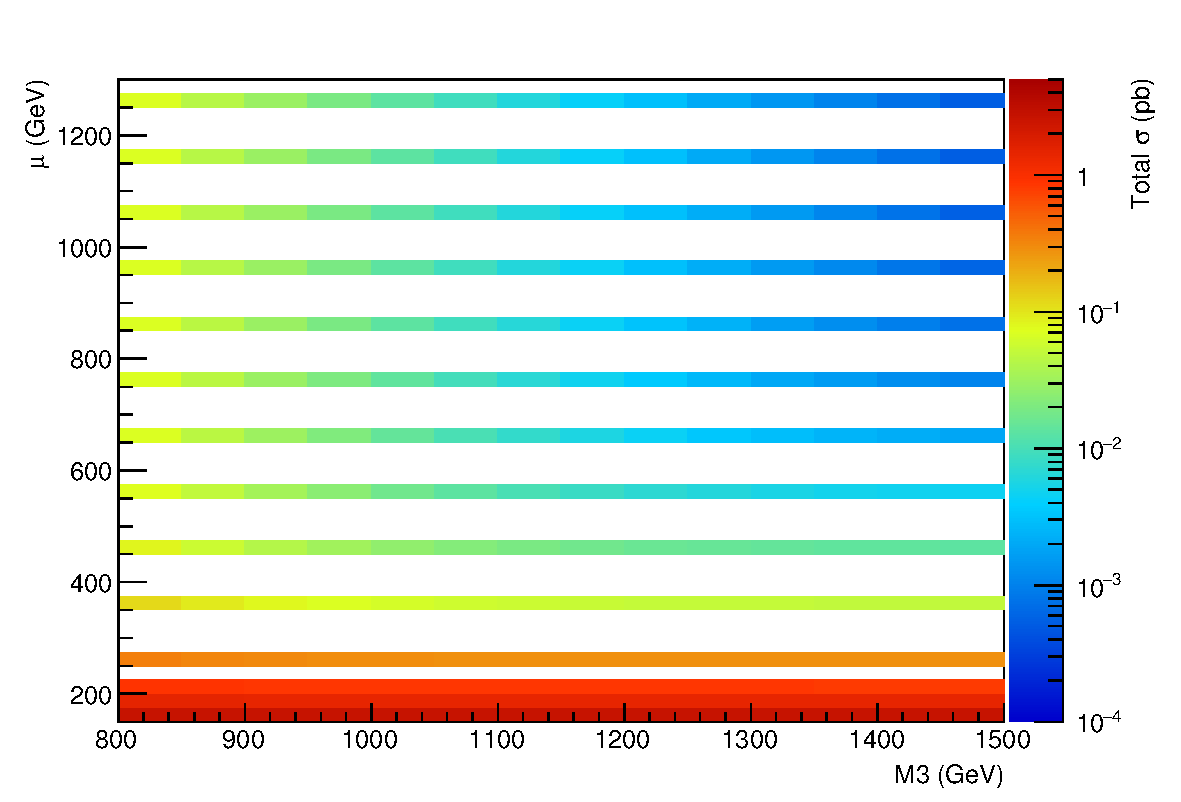
\includegraphics[width=0.49\textwidth]{figures/SigXsec_total}
  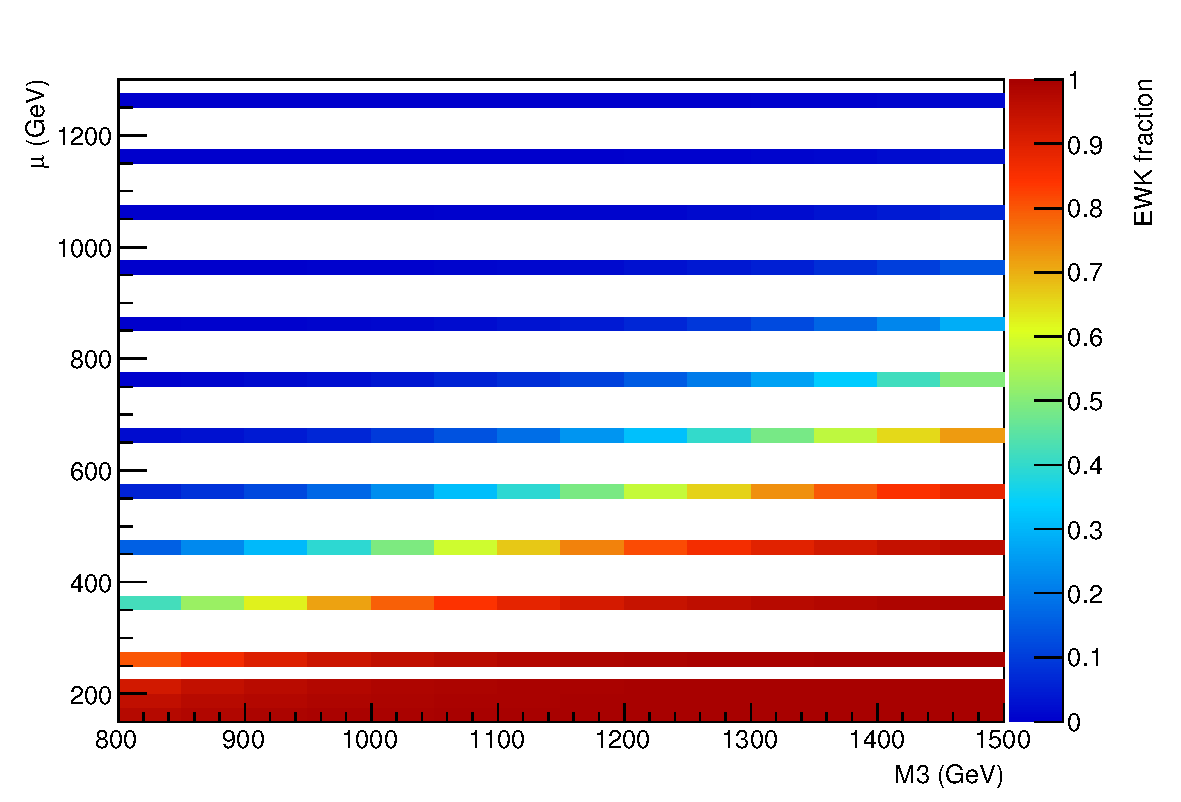
\includegraphics[width=0.49\textwidth]{figures/SigXsec_ewkFrac}
  \caption{Sección eficaz total (izquierda) y fracción relativa
    de producción electrodébil (derecha).}
  \label{fig:signal_xs_total}
\end{figure}

\section{Simulación de los fondos del SM}
\label{sec:bkg_samples}

\newcommand{\mccaption}{Se detallan la sección eficaz a LO para cada modo de decaimiento,
  los factores $k$ (para la normalización NLO) y las eficiencias del filtro,
  así como también la luminosidad integrada correspondiente
  a la estadística total de cada muestra.}


Las muestras de los procesos de fondo contaminante simuladas con MC utilizadas
en este análisis se describen a continuación. Como se discutirá en la
\cref{cap:fondos}, la contaminación de fotones mal identificados
provenientes de jets y electrones es estimada con métodos basados en datos. Sin
embargo, las muestras MC también han sido consideradas en estos casos para los
estudios de optimización y la evaluación de las incertezas sistemáticas.

\subsection{$W/Z$ + $\gamma$}

Se espera que la producción de {\wgam} y {\zgam} sea un fondo importante
para esta búsqueda. Ambas muestras fueron generadas usando el generador
de eventos {\sherpa} v1.4.1\cite{SherpaGen} y
usando las funciones de distribución partónica CT10.
La combinación de los elementos de matriz con las lluvias partónicas
es realizada de acuerdo a un procedimiento mejorado CKKW\cite{Catani:2001cc,Krauss:2002up}.
Un filtro a nivel generados es aplicado requiriendo al menos un fotón
con $\pt > 80(70) \gev$ en el estado final de las muestras de {\wgam} (\zgam).
Todos los decaimientos leptónicos del bosón $Z$ fueron considerados,
incluyendo el decaimiento invisible $Z\to\nu\nu$.
También se tuvo en cuenta un muestra de $V(\to qq)+\gamma\,  (V=W,Z/\gamma*)$
debido a que cierta energía faltante real puede  ser producida en el caso
de decaimientos de sabores pesados.

\begin{table}[!htbp]
  \centering
  \caption{Muestras de W/Z$+\gamma$.
    La sección eficaz a LO se especifica para cada modo de decaimiento,
    al igual que los factores $k$, y las eficiencias del filtro.
    La última columna contiene la luminosidad integrada correspondiente a la estadística total
    de cada muestra.}

  \small
  \begin{tabularx}{\textwidth}{LCRRRR}
    \hline
    Proceso & Generador & $\sigma$ [pb] & Factor-$k$ & Eficiencia & $L$ [\ifb] \\
    \hline
    {\wenugam}    & {\sherpa} &  0.7193  &  1.0  &  1.0  &  695.16 \\
    {\wmunugam}   & {\sherpa} &  0.7178  &  1.0  &  1.0  &  696.56 \\
    {\wtaunugam}  & {\sherpa} &  0.7199  &  1.0  &  1.0  &  694.57 \\
    {\zeegam}     & {\sherpa} &  0.1861  &  1.0  &  1.0  &  1069.53 \\
    {\zmumugam}   & {\sherpa} &  0.1858  &  1.0  &  1.0  &  1076.71 \\
    {\ztautaugam} & {\sherpa} &  0.1858  &  1.0  &  1.0  &  1076.19 \\
    {\znngam}   & {\sherpa} &  0.7625  &  1.0  &  1.0  &  655.74 \\
    {\vqqgam} & {\sherpa}  &  6.756  &  1.0  &  1.0  &  89.0 \\
    \hline
    %% \multicolumn{5}{c}{Variaciones sistemáticas} \\
    %% \hline
    %% {\wenugam} (fact. 0.25x)    & {\sherpa} &  0.7193  &  1.0  &  1.0  &  278.05 \\
    %% {\wenugam} (fact. 4x)       & {\sherpa} &  0.7193  &  1.0  &  1.0  &  278.05 \\
    %% {\wenugam} (renorm. 0.25x)  & {\sherpa} &  0.7193  &  1.0  &  1.0  &  278.05 \\
    %% {\wenugam} (renorm. 4x)     & {\sherpa} &  0.7193  &  1.0  &  1.0  &  278.05 \\
    %% {\wenugam} (ckkw 15)        & {\sherpa} &  0.7193  &  1.0  &  1.0  &  278.05 \\
    %% {\wenugam} (ckkw 30)        & {\sherpa} &  0.7193  &  1.0  &  1.0  &  278.05 \\
    %% {\wmunugam} (fact. 0.25x)   & {\sherpa} &  0.7193  &  1.0  &  1.0  &  278.63 \\
    %% {\wmunugam} (fact. 4x)      & {\sherpa} &  0.7193  &  1.0  &  1.0  &  278.63 \\
    %% {\wmunugam} (renorm. 0.25x) & {\sherpa} &  0.7193  &  1.0  &  1.0  &  278.63 \\
    %% {\wmunugam} (renorm. 4x)    & {\sherpa} &  0.7193  &  1.0  &  1.0  &  278.63 \\
    %% {\wmunugam} (ckkw 15)       & {\sherpa} &  0.7193  &  1.0  &  1.0  &  278.63 \\
    %% {\wmunugam} (ckkw 30)       & {\sherpa} &  0.7193  &  1.0  &  1.0  &  278.63 \\
    %% {\wtaunugam} (fact. 0.25x)  & {\sherpa} &  0.7193  &  1.0  &  1.0  &  277.81 \\
    %% {\wtaunugam} (fact. 4x)     & {\sherpa} &  0.7193  &  1.0  &  1.0  &  277.81 \\
    %% {\wtaunugam} (renorm. 0.25x)& {\sherpa} &  0.7193  &  1.0  &  1.0  &  277.81 \\
    %% {\wtaunugam} (renorm. 4x)   & {\sherpa} &  0.7193  &  1.0  &  1.0  &  277.81 \\
    %% {\wtaunugam} (ckkw 15)      & {\sherpa} &  0.7193  &  1.0  &  1.0  &  277.81 \\
    %% {\wtaunugam} (ckkw 30)      & {\sherpa} &  0.7193  &  1.0  &  1.0  &  277.81 \\
    %% \hline
  \end{tabularx}
  \label{tab:bkg_wzgamma_samples}
\end{table}


\subsection{$W/Z$ + jets}
\label{mc_wzjets}

Se espera que la producción de W$^{\pm}$ y bosones $Z$ en asociación con jets
contribuya a los fondos contaminantes de esta búsqueda, con los fotones provenientes de electrones y jets
mal identificados. Especialmente para los segundos, esta contaminación no está
bien descripta por el MC. Por esta razón se utilizan métodos basados en datos
para estimar su contribución en las diferentes regiones de señal y control, como
se describe en el \cref{cap:fondos}. Varias muestras de MC
fueron consideradas para validar los métodos.

Como se describe en el \cref{cap:seleccion} la selección de señal involucra
muchos jets en el estado final, razón por lo que es importante modelar los estados final
multipartónicos de forma adecuada. Con esto en mente, el generador de eventos
{\alpgen} (v 2.14) fue utilizado, incluyendo los efectos EWK y QCD a LO para los
procesos de interacción fuerte multipartónicos. Se utilizó {\herwig} v6.5.2 para la simulación de las lluvias y los procesos de
fragmentación y {\jimmy} para la simulación de los eventos subyacentes. Las
funciones de densidad partónica utilizadas fueron las CTEQ6L1. La normalización
a la luminosidad integrada acumulada se realizó a partir de la sección eficaz
mostrada en la \cref{tab:bkg_wzjets_samples} usando cálculos QCD a NNLO del
programa FEWZ\cite{Anastasiou:2003ds}. En cada caso los mismos factores de
normalización fueron aplicados a los elementos de matriz de {\alpgen}.

Finalmente, se realizó la remoción de eventos para evitar el conteo doble de
eventos que ya fueron tenidos en cuenta en las muestras de Z$\gamma$ y
W$\gamma$. Para esto, los eventos de $W(Z)+\text{jets}$ con fotones con $\pt>80(70)\gev$ y $\Delta R(\ell/q/g, \gamma) > 0.1$ fueron
removidos de las muestras.

\begin{table}[!htbp]
  \centering
  \caption{Muestras de $W/Z+\text{jets}$. \mccaption}

  \footnotesize
  \begin{tabularx}{\textwidth}{z{4cm}CRy{1.5cm}y{1.5cm}y{1.5cm}}
    \hline
    Proceso & Generador & $\sigma$ [pb] & Factor-$k$ & Eficiencia & $L$ [\ifb] \\
    \hline
    $Z\to ee$            &  \alpgen+\jimmy  & 711.77 & 1.23 & 1.00 & 7.548 \\
    $Z\to ee$ (+ 1 jet)  &  \alpgen+\jimmy  & 155.17 & 1.23 & 1.00 & 6.994 \\
    $Z\to ee$ (+ 2 jets) &  \alpgen+\jimmy  & 48.745 & 1.23 & 1.00 & 6.746 \\
    $Z\to ee$ (+ 3 jets) &  \alpgen+\jimmy  & 14.225 & 1.23 & 1.00 & 6.286 \\
    $Z\to ee$ (+ 4 jets) &  \alpgen+\jimmy  & 3.7595 & 1.23 & 1.00 & 6.487 \\
    $Z\to ee$ (+ 5 jets) &  \alpgen+\jimmy  & 1.0945 & 1.23 & 1.00 & 7.428 \\
    \zmm              &  \alpgen+\jimmy  & 712.11 & 1.23 & 1.00 & 7.557 \\
    \zmm\ (+ 1 jet)   &  \alpgen+\jimmy  & 154.77 & 1.23 & 1.00 & 7.011 \\
    \zmm\ (+ 2 jets)  &  \alpgen+\jimmy  & 48.912 & 1.23 & 1.00 & 6.731 \\
    \zmm\ (+ 3 jets)  &  \alpgen+\jimmy  & 14.226 & 1.23 & 1.00 & 6.286 \\
    \zmm\ (+ 4 jets)  &  \alpgen+\jimmy  & 3.7838 & 1.23 & 1.00 & 6.445 \\
    \zmm\ (+ 5 jets)  &  \alpgen+\jimmy  & 1.1148 & 1.23 & 1.00 & 7.292 \\
    \ztt              & \alpgen+\jimmy  & 711.81 & 1.23 & 1.00 &  7.560 \\
    \ztt\ (+ 1 jet)   & \alpgen+\jimmy  & 155.13 & 1.23 & 1.00 &  6.996 \\
    \ztt\ (+ 2 jets)  & \alpgen+\jimmy  & 48.804 & 1.23 & 1.00 &  6.746 \\
    \ztt\ (+ 3 jets)  & \alpgen+\jimmy  & 14.160 & 1.23 & 1.00 &  6.315 \\
    \ztt\ (+ 4 jets)  & \alpgen+\jimmy  & 3.7744 & 1.23 & 1.00 &  6.462 \\
    \ztt\ (+ 5 jets)  & \alpgen+\jimmy  & 1.1163 & 1.23 & 1.00 &  7.283 \\
    \hline
    \wenu             & \alpgen+\jimmy  & 8037.10  & 1.186 & 1.00 & 0.362 \\
    \wenu\ (+ 1 jet)   & \alpgen+\jimmy  & 1579.20  & 1.186 & 1.00 & 1.334 \\
    \wenu\ (+ 2 jets)  & \alpgen+\jimmy  & 477.20   & 1.186 & 1.00 & 6.661 \\
    \wenu\ (+ 3 jets)  & \alpgen+\jimmy  & 133.93   & 1.186 & 1.00 & 6.358 \\
    \wenu\ (+ 4 jets)  & \alpgen+\jimmy  & 35.62    & 1.186 & 1.00 & 5.917 \\
    \wenu\ (+ 5 jets)  & \alpgen+\jimmy  & 10.55    & 1.186 & 1.00 & 5.592 \\
    \wmnu             & \alpgen+\jimmy  & 8040.00  & 1.186 & 1.00 & 0.363 \\
    \wmnu\ (+ 1 jet)  & \alpgen+\jimmy  & 1580.30  & 1.186 & 1.00 & 1.333 \\
    \wmnu\ (+ 2 jets) & \alpgen+\jimmy  & 477.50   & 1.186 & 1.00 & 6.656 \\
    \wmnu\ (+ 3 jets) & \alpgen+\jimmy  & 133.94   & 1.186 & 1.00 & 6.357 \\
    \wmnu\ (+ 4 jets) & \alpgen+\jimmy  & 35.64    & 1.186 & 1.00 & 6.033 \\
    \wmnu\ (+ 5 jets) & \alpgen+\jimmy  & 10.57    & 1.186 & 1.00 & 1.595 \\
    \wtnu             & \alpgen+\jimmy  & 8035.80  & 1.186 & 1.00 & 0.353 \\
    \wtnu\ (+ 1 jet)  & \alpgen+\jimmy  & 1579.80  & 1.186 & 1.00 & 1.307 \\
    \wtnu\ (+ 2 jets) & \alpgen+\jimmy  & 477.55   & 1.186 & 1.00 & 6.567 \\
    \wtnu\ (+ 3 jets) & \alpgen+\jimmy  & 133.79   & 1.186 & 1.00 & 6.365 \\
    \wtnu\ (+ 4 jets) & \alpgen+\jimmy  & 35.58    & 1.186 & 1.00 & 5.921 \\
    \wtnu\ (+ 5 jets) & \alpgen+\jimmy  & 10.54    & 1.186 & 1.00 & 5.199 \\
    \hline
  \end{tabularx}
  \label{tab:bkg_wzjets_samples}
\end{table}


\subsection{Pares de \emph{tops} (+ $\gam$)}
\label{sec:mcttbargam}

Otro fondo importante para este análisis es el {\ttgam}. Esta muestra fue
generada utilizando {\madgraph}\cite{Alwall:2007st} y la PDF CTEQ6L1.
{\pythiasix}\cite{pythia} fue usado para la simulación de las lluvias
partónicas, fragmentación y eventos subyacentes. La radiación de fotones fue
agregadas utilizando {\photos}\cite{photos}, y los decaimientos de los leptones
tau con {\tauola}\cite{tauola}. Se requirió que los fotones a nivel generador
tengan un $\pt > 80 \gev$. Para evitar efectos cinemáticos introducidos por el
filtro, el corte en el {\pt} del fotón en la muestra reconstruida se aumentó a
95 {\gev}. Se utilizó un factor-$k$ de $1.9 \pm 0.4$\cite{Melnikov:2011ta, tth}
para tener en cuenta efectos de mayor orden en teoría de perturbaciones.
Los detalles de la simulación se encuentran en la \cref{tab:mc_ttbar_samples}.
Se utilizaron además algunas muestras a nivel generador como variaciones para calcular
las incertezas sistemáticas como se explica en la \cref{sec:syst_ttbargamma}.

La producción de {\ttbar}, donde los electrones o los jets son mal identificados
como fotones es una fuente de fondo que debe ser considerado. Aunque ambas
contaminaciones fueron estimadas a partir de los datos, se utilizaron eventos simulados
en la etapa de optimización y para realizar chequeos de los métodos utilizados.
La
muestra MC fue generada utilizando
{\powheg}\cite{Nason:2004rx,Frixione:2007vw,Alioli:2010xd} con la lluvia
partónica y fragmentación hecha por {\pythia}. Para el UE se utilizó Perugia
2011C con el
conjunto de PDFs CTEQ6L1 LO. La radiación de fotones adicional fue agregada con
{\photos}\cite{photos}.

Por último, se realizó la remoción
de los eventos con un fotón real con $\pt > 95 \gev$ y $\Delta R(\ell/g/q,\gamma) > 0.1$ de la muestra de {\ttbar} para evitar la superposición con los eventos
considerados en las muestras de {\ttgam}.


\begin{table}[!htb]
  \centering
  \caption{Muestras de {\ttgam}. {\mccaption}}

  \small
  \begin{tabularx}{\textwidth}{LCRRRR}
    \hline
    Proceso & Generador & $\sigma$ [pb] & Factor-$k$ & Eficiencia & $L$ [\ifb] \\
    \hline
    {\ttbar} & \powheg+\pythia & 253.00 & 1.00 & 0.543 & 580 \\
    \hline
    %    \ttbargam noAllHad \madgraph (164439) & 0.092363 & 1.9 & 1 & 1139.7 \\
    {\ttgam} (lep) & \madgraph & 0.09873 & 1.90 & 1.00 & 1066.2 \\
    {\ttgam} (had) & \madgraph  & 0.068599 & 1.90 & 1.00 & 1534.5 \\
    \hline
    %% \multicolumn{6}{c}{Variaciones sistematicas} \\
    %% \hline
    %%     {\ttgam} (lep) (scale$^{+}$) & \madgraph & 0.09873 & 1.9 & 1 & 1066.2 \\
    %%     {\ttgam} (lep) (scale$^{-}$) & \madgraph & 0.09873 & 1.9 & 1 & 1066.2 \\
    %%     {\ttgam} (lep) ($\alphas^{+}$)  & \madgraph & 0.09873 & 1.9 & 1 & 1066.2 \\
    %%     {\ttgam} (lep) ($\alphas^{-}$)  & \madgraph & 0.09873 & 1.9 & 1 & 1066.2 \\
    %%     {\ttgam} (lep) (FSR$^{+}$) & \madgraph & 0.09873 & 1.9 & 1 & 1066.2 \\
    %%     {\ttgam} (lep) (FSR$^{-}$) & \madgraph & 0.09873 & 1.9 & 1 & 1066.2 \\
    %% \hline
  \end{tabularx}
  \label{tab:mc_ttbar_samples}
\end{table}

\subsection{\emph{Top} (+ $\gamma$)}

La producción de un quark \emph{top} con un fotón asociado fue generado utilizando
\textsc{Whizard} 2.1.1 \cite{whizard, whizard2}.
El fotón extra puede estar tanto en la producción del \emph{top} como en los decaimientos
sucesivos. Sin embargo, la producción y el decaimiento son tratados de forma
separada, por lo que los efectos de interferencia pueden ser ignorados. Para las
lluvias partónicas y la fragmentación fue utilizado {\pythia}\cite{pythia}. La
radiación de fotones fue agregada con {\photos}\cite{photos}, y los
decaimientos de los leptones tau con {\tauola}\cite{tauola}.

La producción de \emph{tops} resulta en un fondo poco importante para este análisis,
aunque de mayor importancia para las regiones de control y validación. La producción $Wt$
fue generada utilizando {\powheg}, incluyendo correcciones a NLO en QCD. La lluvia
partónica y la fragmentación fue simulada utilizando {\pythia} (con P2011).
Se utilizó el conjunto de PDFs CT10. Las muestras fueron normalizadas con
la sección eficaz calculada en \cite{Kidonakis:2010ux}.

%%Para la produccion en el canal $t$, las muestras MC
%% production, the MC samples with sample ID 110101 were used, with the
%% $W$ boson decaying leptonically. These were generated with
%% \acermc \cite{acer}, with parton showering and fragmentation performed
%% by {\pythia} with the P2011C tune and CTEQ6L1 PDF set.  The samples were
%% scaled to the cross section calculated by \cite{Kidonakis:2011wy}.
%% Single top produced by $s$-channel was not used because it was found
%% to be negligible.
%%Se removieron los  Overlap between the single top and single top $\gamma$ samples has been removed.

\begin{table}[!htb]
  \centering
  \caption{Muestras de quark \emph{top} + \gam. La sección eficaz a
    NNLO, eficiencia del filtro, y luminosidad integrada correspondiente a la estadística total de cada muestra
    están detalladas en la tabla.}

  \small
  \begin{tabularx}{\textwidth}{Lx{2.8cm}y{1.5cm}y{1.5cm}y{1.5cm}}
    \hline
    Proceso & Generador & $\sigma$ [pb] & Eficiencia & $L$ [\ifb] \\
    \hline
    \emph{top} + $\gamma$ (en producción) & \wizhard+\pythia   & 0.187298 & 0.121980 & 4810 \\
    \emph{top} + $\gamma$ (en decaimiento) & \wizhard+\pythia   & 0.313866 & 0.012927 & 4930 \\
    \hline
    $tW$ (lep) + $\gamma$ (en producción)                             & \wizhard+\pythia          & 0.01292  & 0.16437 & 4710 \\
    $tW$ (lep) + $\gamma$ (en decaimiento del $t$)             & \wizhard+\pythia     & 0.01454  & 0.02875 & 12000 \\
    $tW$ (lep) + $\gamma$ (en decaimiento del $W$)                    & \wizhard+\pythia     & 0.01041  & 0.07549 & 6370 \\
    $t$(lep)$W$(had) + $\gamma$ (en producción)                 & \wizhard+\pythia        & 0.02583  & 0.16244 & 4770 \\
    $t$(lep)$W$(had) + $\gamma$ (en decaimiento del $t$) & \wizhard+\pythia   & 0.02908  & 0.02761 & 6230 \\
    $t$(lep)$W$(had) + $\gamma$ (en decaimiento del $W$)        & \wizhard+\pythia   & 0.01159  & 0.06471 & 6660 \\
    $t$(had)$W$(lep) + $\gamma$ (en producción)                 & \wizhard+\pythia      & 0.02582  & 0.16178 & 4790 \\
    $t$(had)$W$(lep) + $\gamma$ (en decaimiento del $t$) & \wizhard+\pythia   & 0.02013  & 0.04198 & 5920 \\
    $t$(had)$W$(lep) + $\gamma$ (en decaimiento del $W$)        & \wizhard+\pythia   & 0.02079  & 0.07574 & 3180 \\
    \hline
  \end{tabularx}
  \label{tab:bkg_st_samples}
\end{table}


\subsection{{\gjet} y multijets}

La contaminación debido a la producción QCD de fotones directos y multijets,
es en todos los casos el resultado de eventos patológicos
(jets mal identificados como fotones, y jets o fotones mal reconstruidos dejando
una alta cantidad de energía faltante). Sin embargo, no se espera que sea un
fondo dominante en el espacio de fase explorado en este análisis. La
contribución de eventos con jets mal identificados como fotones se estima a
partir de los datos en la \cref{sec:jfakes}.

Las muestras de multijets listadas en la \cref{tab:bkg_qcd_samples} fueron
utilizadas para el proceso de optimización y estudios de sensibilidad
preliminares. La producción de fotones directos fue simulada con {\sherpa}
v1.4.1\cite{SherpaGen}, con hasta cuatro partones en la ME+PS y usando el
conjunto de PDFs CT10. El espectro inclusivo se dividió en diversas muestras con
diferentes umbrales de {\pt} del fotón para optimizar la generación de eventos.

Muestras alternativas fueron utilizadas para la estimación de las incertezas
sistemáticas, generadas con {\pythiaeight} (usando CTEQ6L1) y {\alpgen} v2.14
(con la misma configuración que los eventos de $W/Z +$ jets descriptos en
\cref{mc_wzjets}). Los detalles pueden verse en la \cref{tab:bkg_qcd_samples}.

\begin{table}[ht!]
  \centering
  \caption{Muestras de QCD {\gjet} y multijet utilizadas en este análisis.
    La sección eficaz a LO para cada modo de decaimiento,
    y las eficiencias del filtro están detalladas,
    así como también la luminosidad integrada correspondiente a la estadística
    total de cada muestra.}

  \small
   \begin{tabularx}{\textwidth}{z{5.5cm}CRRR}
    \hline
    Proceso & Generador & $\sigma$ [pb] & Eficiencia & $L$ [\ifb] \\
    \hline
    {\gjet} ($\pt^\gamma>70\gev$)   & {\sherpa} &    2153.0  &  1.0  &  1.160 \\
    {\gjet} ($\pt^\gamma>140\gev$)  & {\sherpa} &    137.85  &  1.0  &  10.881 \\
    {\gjet} ($\pt^\gamma>280\gev$)  & {\sherpa} &     5.963  &  1.0  &  167.657 \\
    {\gjet} ($\pt^\gamma>500\gev$)  & {\sherpa} &     0.276  &  1.0  &  3617.291 \\
    {\gjet} ($\pt^\gamma>800\gev$)  & {\sherpa} &    0.0133  &  1.0  &  7492.807 \\
    {\gjet} ($\pt^\gamma>1000\gev$) & {\sherpa} &   0.00238  &  1.0  &  41980.269 \\
    \hline
    {\gjet} ($\pt^\gamma>70\gev$)   & {\pythiaeight} &   3425000  &  $0.00057$  &  1535.4  \\
    {\gjet} ($\pt^\gamma>140\gev$)  & {\pythiaeight} &    122170  &  $0.00097$  &  8449.2 \\
    {\gjet} ($\pt^\gamma>280\gev$)  & {\pythiaeight} &    3348.7  &  $0.00145$ &  206559.7 \\
    {\gjet} ($\pt^\gamma>500\gev$)  & {\pythiaeight} &    115.63  &  $0.0018$  &  4789097.0\\

    %% \hline
    %% \gjetnj{1} ($\pt>70\gev$)   & {\alpgen}+{\jimmy} &   577.480  &  1.0  &  0.147 \\
    %% \gjetnj{1} ($\pt>140\gev$)  & {\alpgen}+{\jimmy} &   26.198   &  1.0  &  3.626 \\
    %% \gjetnj{1} ($\pt>280\gev$)  & {\alpgen}+{\jimmy} &   0.83119  &  1.0  &  30.077 \\
    %% \gjetnj{1} ($\pt>500\gev$)  & {\alpgen}+{\jimmy} &   0.02914  &  1.0  &  343.159 \\

    %% % \gjetnj{2} ($\ptgam>35\gev$) \alpgen+\jimmy  ( 156846 ) &  4515.0  &  1.0  &  0.00886 \\
    %% \gjetnj{2} ($\pt>70\gev$)    & {\alpgen}+{\jimmy} &   571.870  &  1.0  &  0.175 \\
    %% \gjetnj{2} ($\pt>140\gev$)   & {\alpgen}+{\jimmy} &   38.67100  &  1.0  &  3.879 \\
    %% \gjetnj{2} ($\pt>280\gev$)   & {\alpgen}+{\jimmy} &   1.6811  &  1.0  &  29.741 \\
    %% \gjetnj{2} ($\pt>500\gev$)   & {\alpgen}+{\jimmy} &   0.075517  &  1.0  &  264.841 \\

    %% % \gjetnj{3} ($\ptgam>35\gev$) \alpgen+\jimmy  ( 156851 ) &  1717.0  &  1.0  &  0.00874 \\
    %% \gjetnj{3} ($\pt>70\gev$)  & {\alpgen}+{\jimmy} &   306.10  &  1.0  &  0.049\\
    %% \gjetnj{3} ($\pt>140\gev$) & {\alpgen}+{\jimmy} &   28.57  &  1.0  &  5.250 \\
    %% \gjetnj{3} ($\pt>280\gev$) & {\alpgen}+{\jimmy} &   1.538  &  1.0  &  32.503 \\
    %% \gjetnj{3} ($\pt>500\gev$) & {\alpgen}+{\jimmy} &   0.07707  &  1.0  &  77.822 \\

    %% % \gjetnj{4} ($\ptgam>35\gev$) \alpgen+\jimmy  ( 156856 ) &  513.940002  &  1.0  &  0.00778 \\
    %% \gjetnj{4} ($\pt>70\gev$)    & {\alpgen}+{\jimmy} &   115.850  &  1.0  &  0.216 \\
    %% \gjetnj{4} ($\pt>140\gev$)   & {\alpgen}+{\jimmy} &   14.216  &  1.0  &  11.951 \\
    %% \gjetnj{4} ($\pt>280\gev$)   & {\alpgen}+{\jimmy} &   0.9185  &  1.0  &  48.992 \\
    %% \gjetnj{4} ($\pt>500\gev$)   & {\alpgen}+{\jimmy} &   0.0512  &  1.0  &  156.354 \\

    %% % \gjetnj{5} ($\ptgam>35\gev$) \alpgen+\jimmy  ( 156861 ) &  163.800003  &  1.0  &  0.0458 \\
    %% \gjetnj{5} ($\pt>70\gev$)    & {\alpgen}+{\jimmy} &   7.00  &  1.0  &  18.569 \\
    %% \gjetnj{5} ($\pt>140\gev$)   & {\alpgen}+{\jimmy} &   0.542  &  1.0  &  92.304 \\
    %% \gjetnj{5} ($\pt>280\gev$)   & {\alpgen}+{\jimmy} &   0.0333  &  1.0  &  450.911 \\
    %% \gjetnj{5} ($\pt>500\gev$)   & {\alpgen}+{\jimmy} &   44.334  &  1.0  &  0.970 \\

    \hline
    Multijet ($\pt^{\mathrm{jet}} \in [20, 80] \gev$)     & {\pythia} &   $7.285 \cdot 10^{10}$ &  0.000129 & 0.00016 \\
    Multijet ($\pt^{\mathrm{jet}} \in [80, 200] \gev$)    & {\pythia} &   $2.634 \cdot 10^{7}$ &  0.003894 & 0.0142 \\
    Multijet ($\pt^{\mathrm{jet}} \in [200,500] \gev$)    & {\pythia} &   $5.442 \cdot 10^{5}$ &  0.001219 & 2.26 \\
    Multijet ($\pt^{\mathrm{jet}} \in [500,1000] \gev$)   & {\pythia} &   $0.006445$ &  0.000708 & 328 \\
    Multijet ($\pt^{\mathrm{jet}} \in [1000,1500] \gev$)  & {\pythia} &   39.74 &  0.002152 & 17400 \\
    Multijet ($\pt^{\mathrm{jet}} \in [1500,2000] \gev$)  & {\pythia} &   0.4161 &  0.004684 & $7.68 \cdot 10^{5}$ \\
    Multijet ($\pt^{\mathrm{jet}} > 2000 \gev$)           & {\pythia} &   0.04064 &  0.0146 & $2.52\cdot 10^{6}$ \\
    \hline
  \end{tabularx}
  \label{tab:bkg_qcd_samples}
\end{table}

\subsection{Diboson}

Los procesos de diboson (WW, WZ, y ZZ) fueron generados utilizando
{\sherpa} y usando la PDF CT10, con la sección eficaz provista por
MCFM\cite{Campbell:2011bn}. Solo los decaimientos leptónicos para
ambos bosones fueron considerados.

\begin{table}[ht!]
  \centering
  \caption{Muestras de Diboson.
    La sección eficaz a LO para cada modo de decaimiento, los factores $k$
    (para la normalización NLO) y las eficiencias del filtro están detalladas,
    así como también la luminosidad integrada correspondiente a la estadística
    total de cada muestra.}

  \small
  \begin{tabularx}{\textwidth}{LCRRRR}
    \hline
    Proceso & Generador & $\sigma$ [pb] & Factor-$k$ & Eficiencia & $L$ [\ifb] \\
    \hline
    %% $WW(2l2\nu)$ \sherpa (126892)  & 5.50 & 1.07 & 1 & 458.9 \\
    %% $WZ(3l)$ \sherpa (126893) & 9.75 & 1.06 & 1 & 261.1 \\
    %% $ZZ(4\ell)$ \sherpa (126894)  & 8.74 & 1.11 & 1  &  185.6 \\
    %% $ZZ(2\ell2\nu)$ \sherpa (126895)  & 0.50 & 1.14 & 1 &  1590.8 \\
    $WW (\to \ell\ell\nu\nu)$     & {\sherpa}  & 5.296  & 1.06 & 1.00 & 1400 \\
    $ZZ (\to \ell\ell\nu\nu)$     & {\sherpa}  & 0.494  & 1.05 & 1.00 & 1700 \\
    $WZ (\to \ell\ell\ell\nu)$    & {\sherpa}  & 9.745  & 1.05 & 1.00 & 260 \\
    $WZ (\to \ell\nu\nu\nu)$      & {\sherpa}  & 1.406  & 1.05 & 1.00 & 270 \\
    $ZW (\to eeqq)$               & {\sherpa}  & 1.465  & 1.05 & 1.00 & 110 \\
    $ZZ (\to eeqq)$               & {\sherpa}  & 0.247  & 1.00 & 1.00 & 120 \\
    $ZW (\to \mu\mu qq)$          & {\sherpa}  & 1.463  & 1.05 & 1.00 & 110 \\
    $ZZ (\to \mu\mu qq)$          & {\sherpa}  & 0.248  & 1.00 & 1.00 & 120 \\
    $ZW (\to \tau\tau qq)$        & {\sherpa}  & 1.452  & 1.05 & 1.00 & 120 \\
    $ZZ (\to \tau\tau qq)$        & {\sherpa}  & 0.242  & 1.00 & 1.00 & 120 \\
    $ZW (\to \nu\nu qq)$          & {\sherpa}  & 2.697  & 1.05 & 1.00 & 64 \\
    $ZZ (\to \nu\nu qq)$          & {\sherpa}  & 1.744  & 1.00 & 1.00 & 69 \\
    $WW (\to e\nu qq)$            & {\sherpa}  & 7.285  & 1.06 & 1.00 & 100 \\
    $WZ (\to e\nu qq)$            & {\sherpa}  & 1.904  & 1.05 & 1.00 & 110 \\
    $WW (\to \mu\nu qq)$          & {\sherpa}  & 7.297  & 1.06 & 1.00 & 100 \\
    $WZ (\to \mu\nu qq)$          & {\sherpa}  & 1.906  & 1.05 & 1.00 & 100 \\
    $WW (\to \tau\nu qq)$         & {\sherpa}  & 7.274  & 1.06 & 1.00 & 100 \\
    $WZ (\to \tau\nu qq)$         & {\sherpa}  & 1.915  & 1.05 & 1.00 & 100 \\
    \hline
  \end{tabularx}
  \label{tab:bkg_diboson_samples}
 \end{table}



%% Referencias
\nocite{Seymour:2013ega}

